\documentclass{article}
\usepackage[utf8]{inputenc}
\usepackage[total={8in,10in}]{geometry}
\usepackage{graphicx}
\graphicspath{{../plots/}}
\usepackage[font=large,labelfont=bf]{caption}
\captionsetup{width=\linewidth}
\usepackage{subcaption}

\begin{document}
	
	\begin{figure}
		\centering
		\begin{subfigure} {.5\columnwidth}
				\centering 
				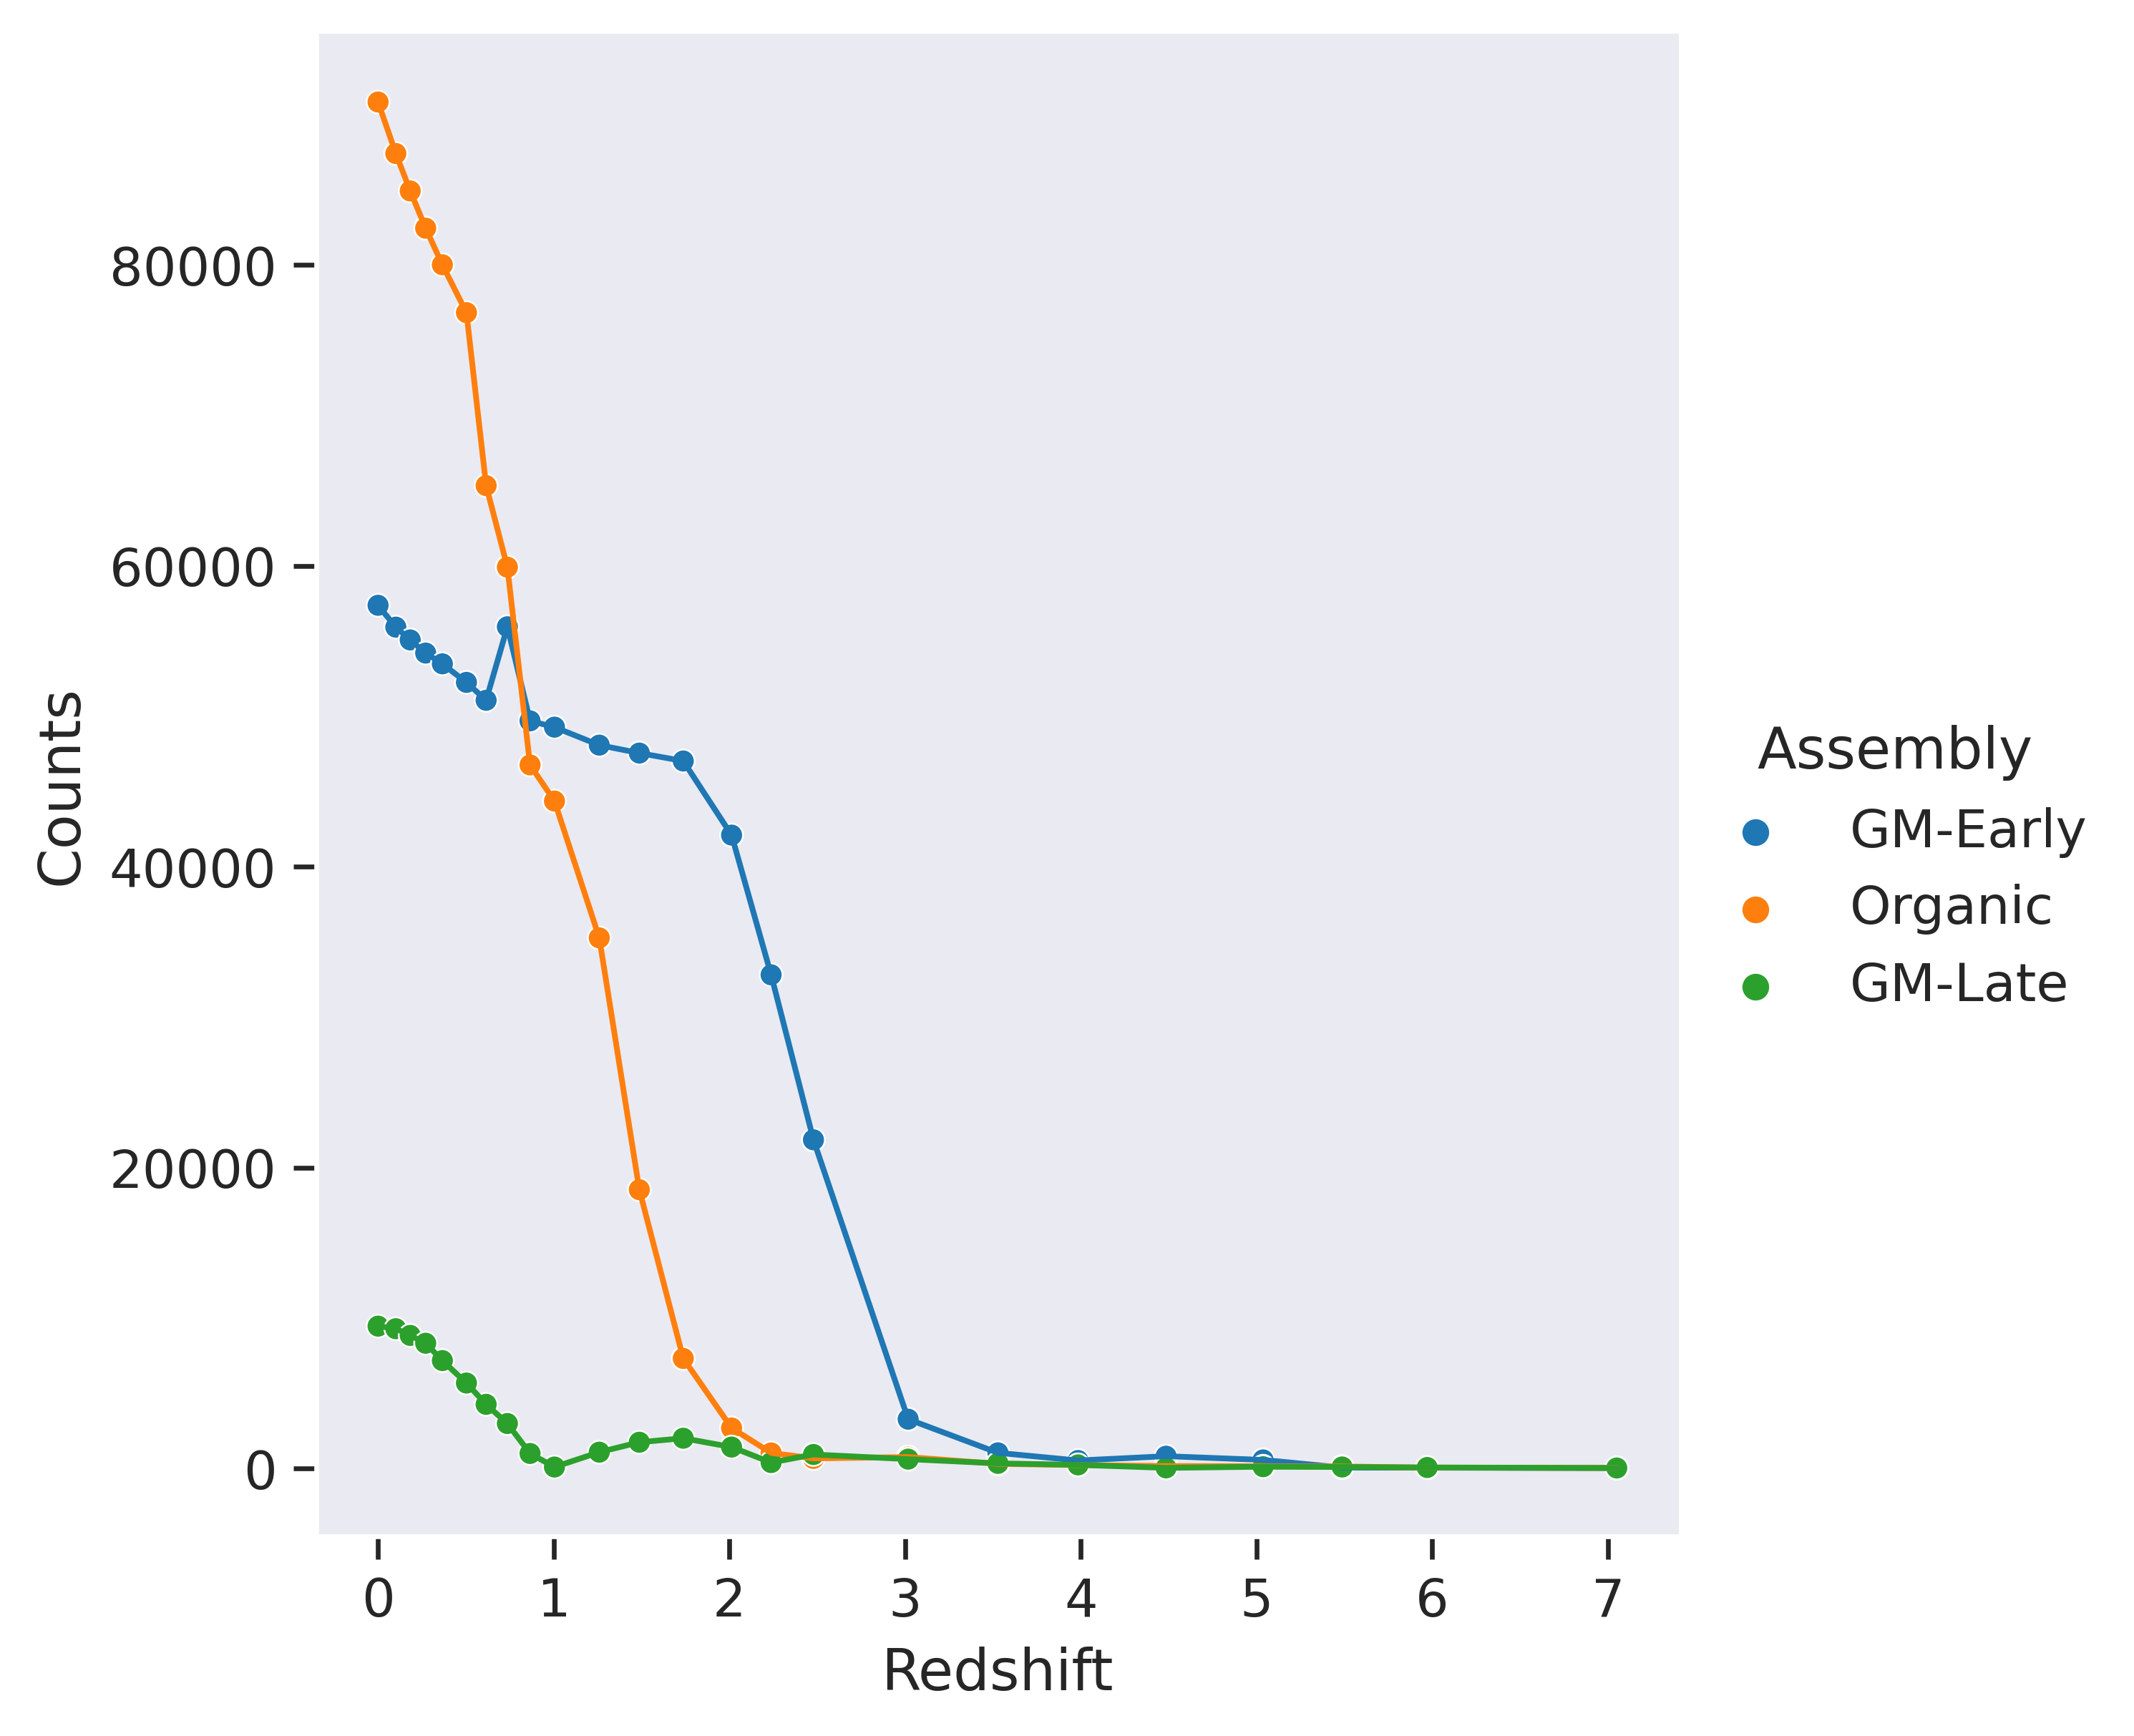
\includegraphics[width=\columnwidth]{../plots/particle_distribution_wrt_redshift.png}
				\caption{Distribution of particles with redshift for three assembly modes.}
		\end{subfigure}
			\hfill
		\begin{subfigure} {.45\columnwidth}
				\centering 
				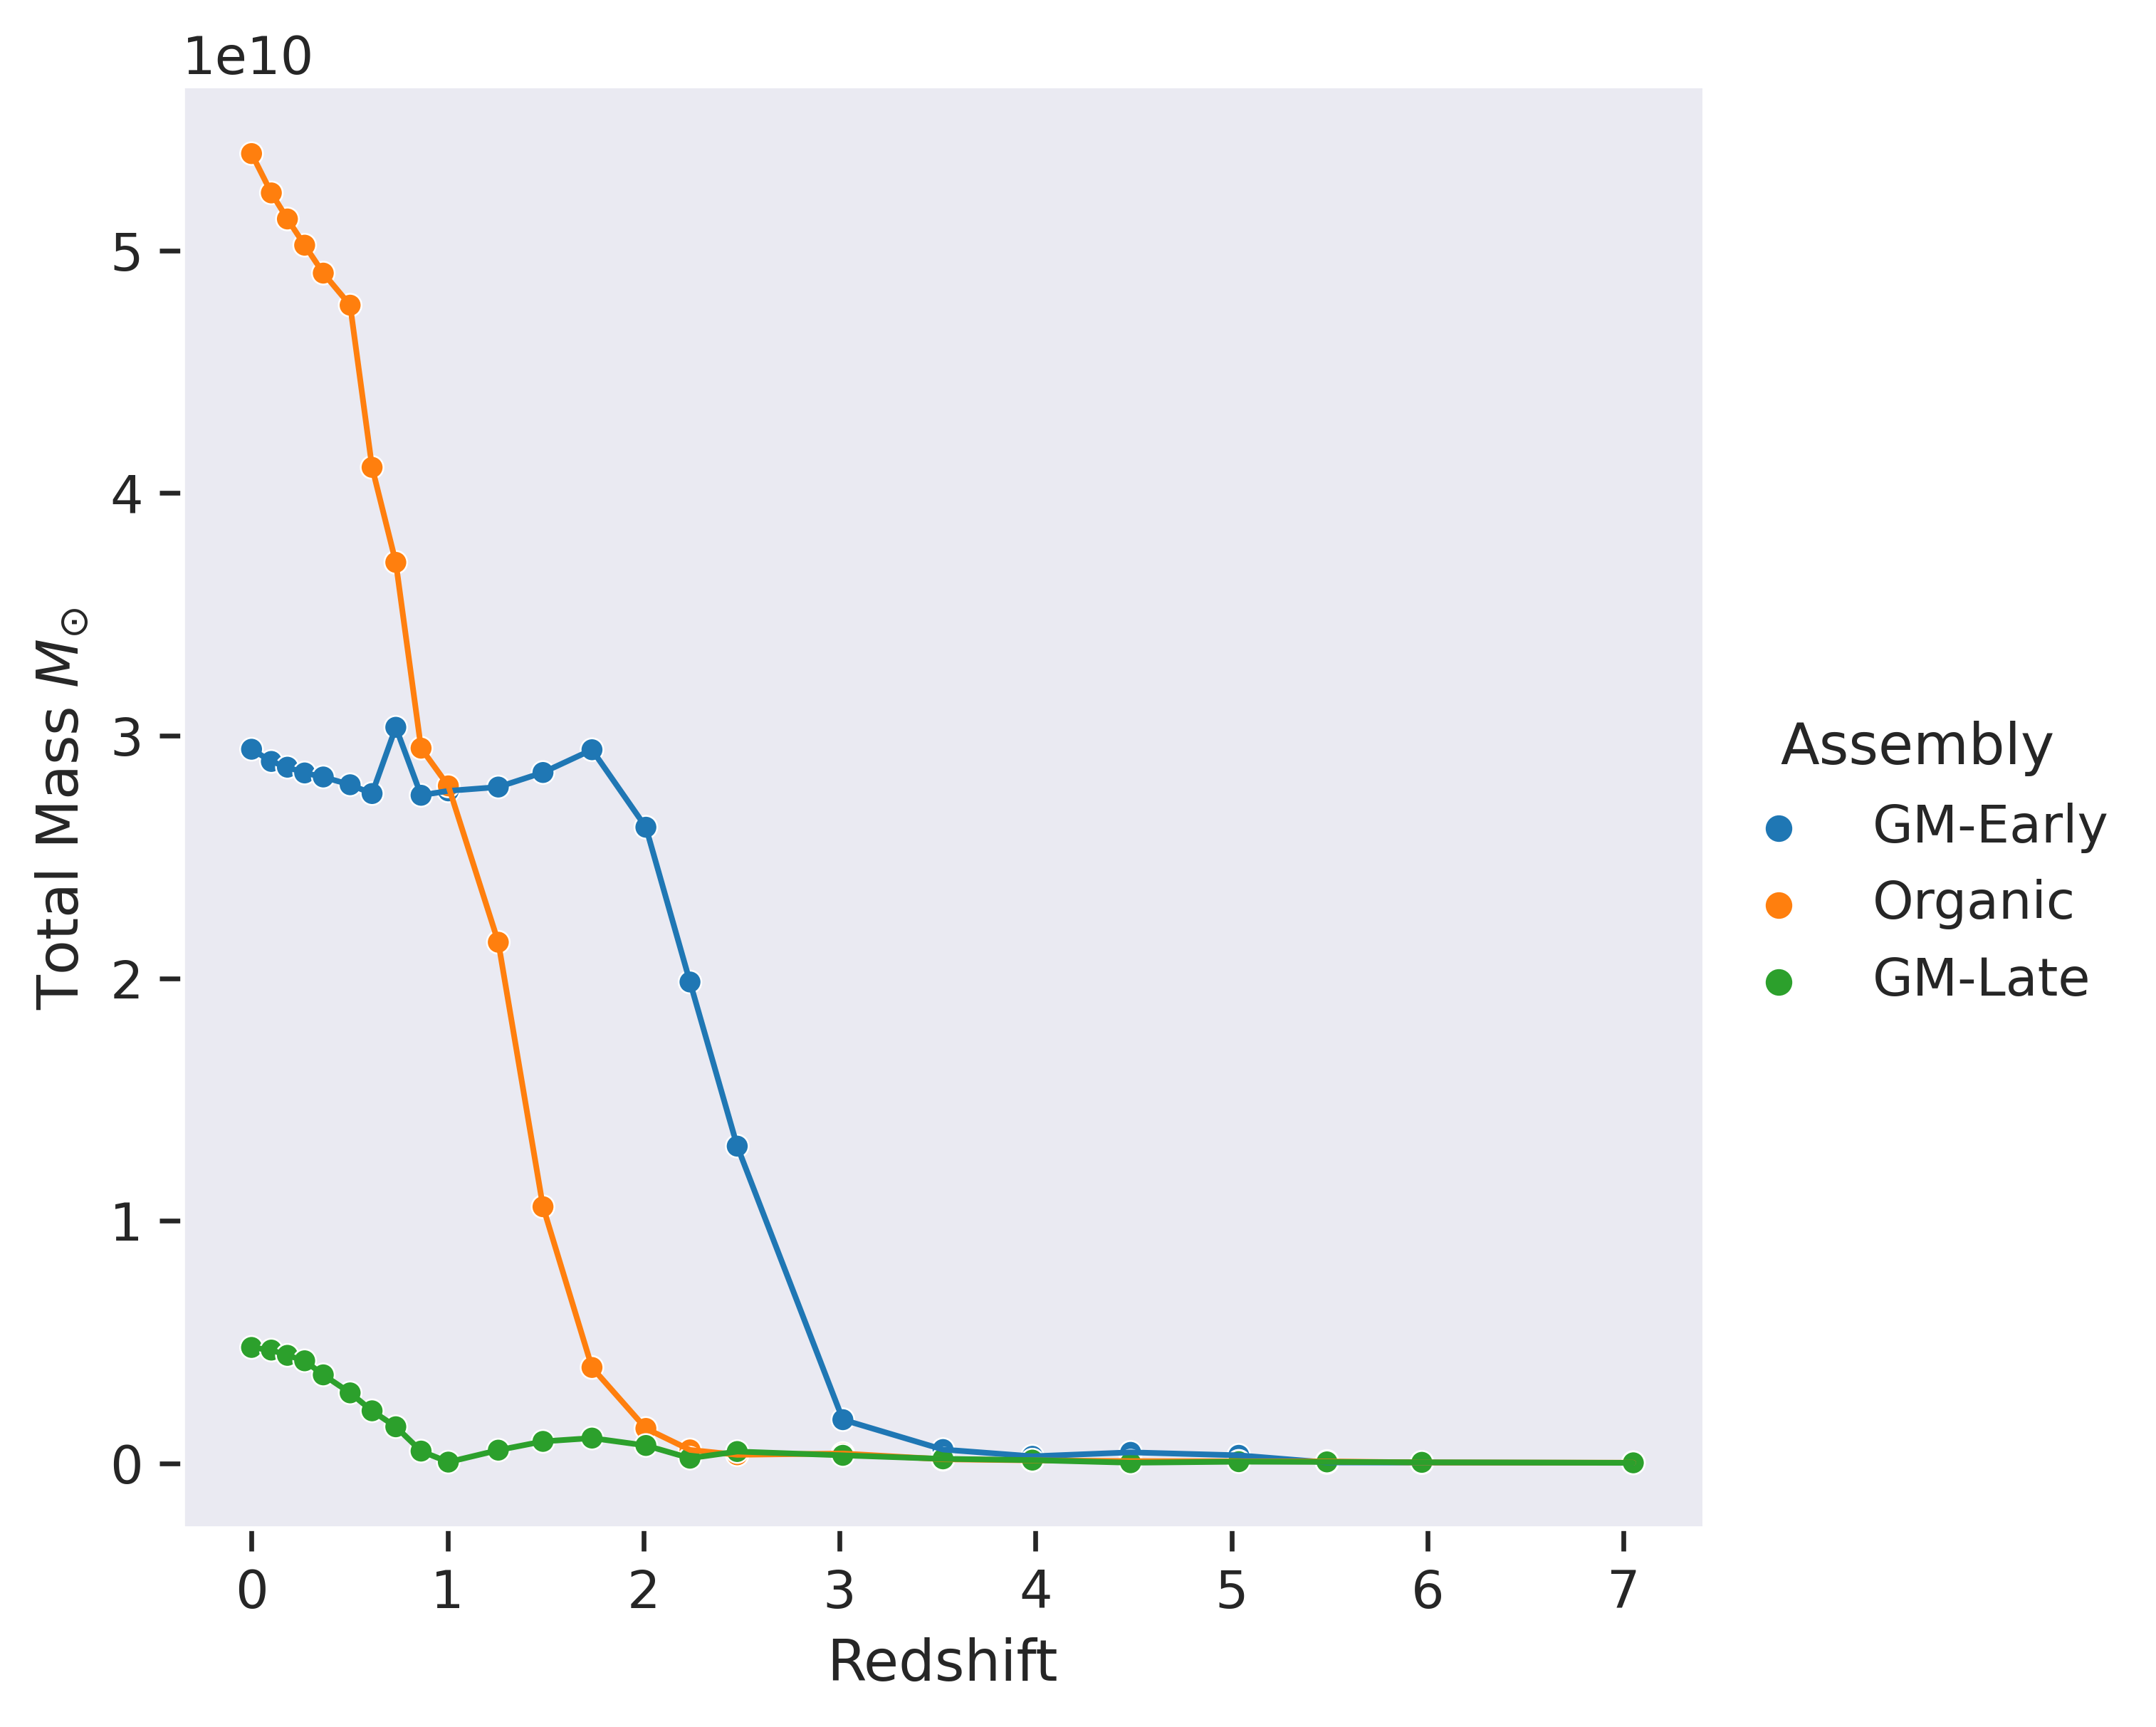
\includegraphics[width=\columnwidth]{../plots/total_mass_wrt_redshift.png}
				\caption{Distribution of total mass of particles with redshift for three assembly modes.}
		\end{subfigure}
		\caption{Evolution of distributions of number of particles and total amount of mass contained in them with redshift for three assembly modes.}
	\end{figure}

	\begin{figure}
			\centering 
			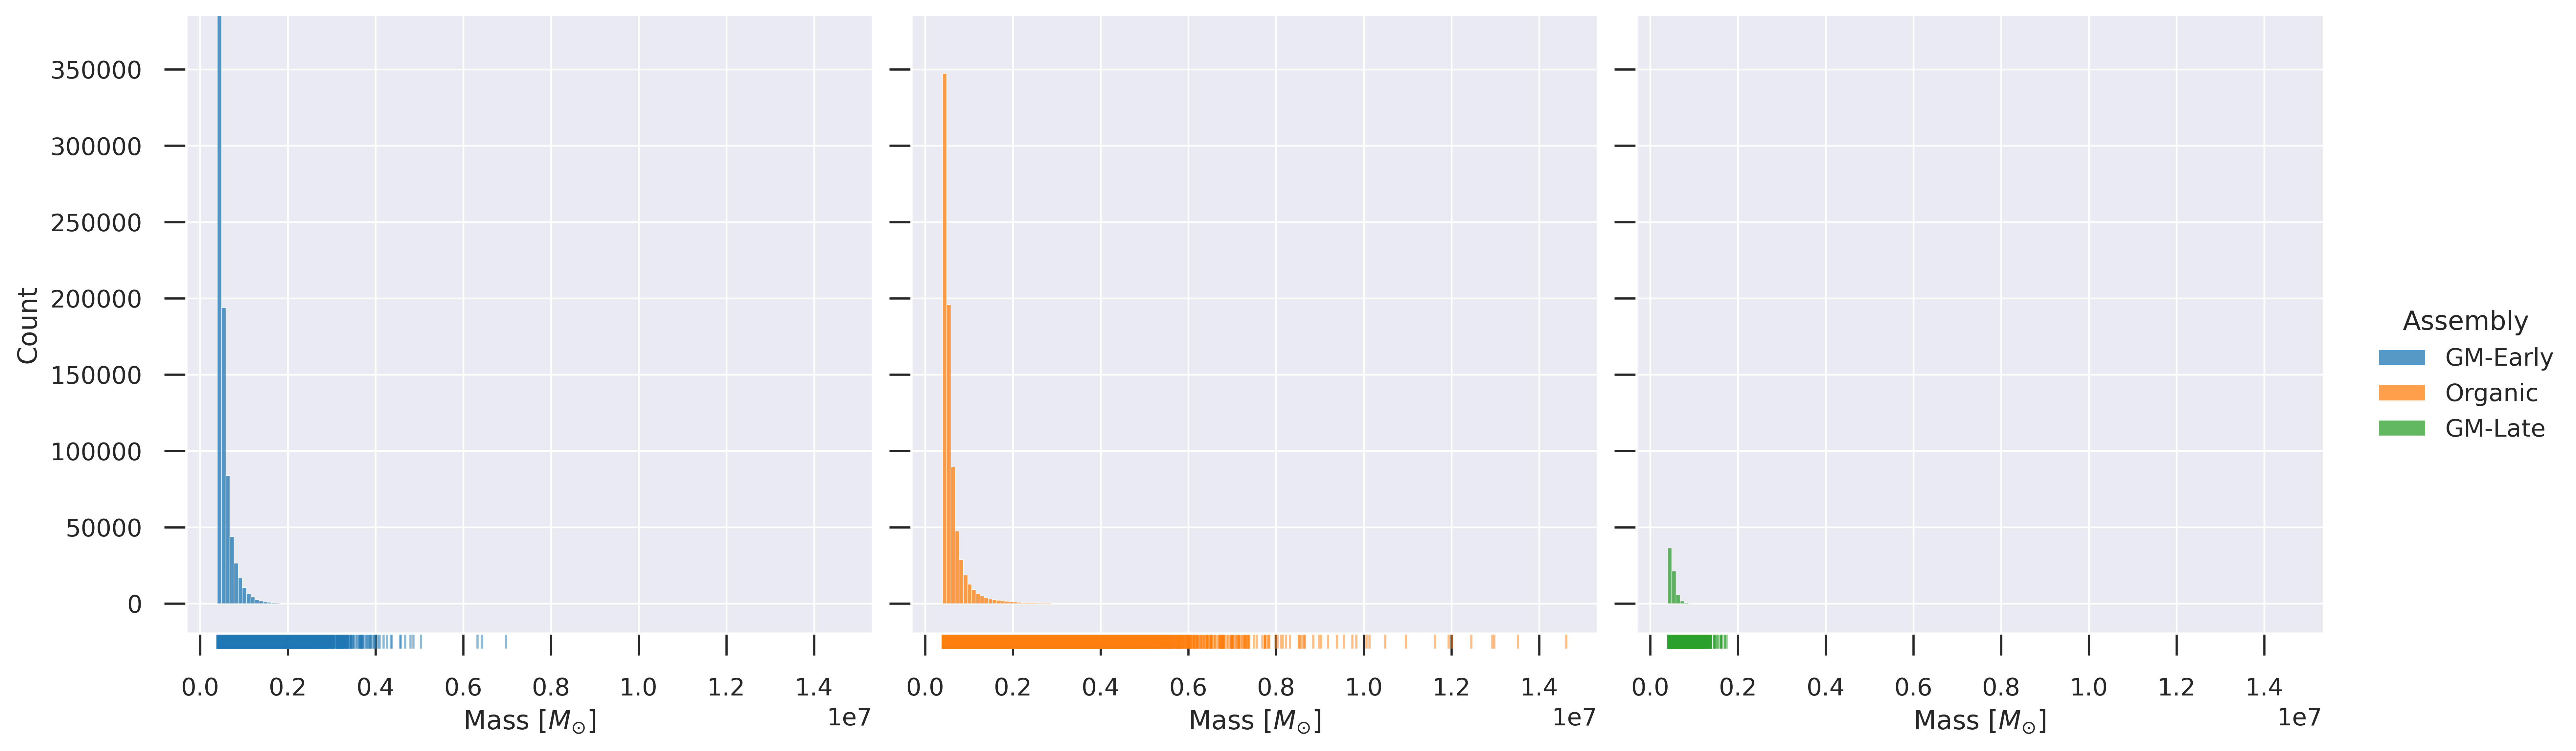
\includegraphics[width=\columnwidth]{../plots/particle_mass_distribution.png}
			\caption{Particles mass distribution combined at all redshifts for three assembly modes. Rugplots on x-axes give an estimate of range of masses involved in the three modes.}
	\end{figure}

	\clearpage

	\begin{figure}
			\centering 
			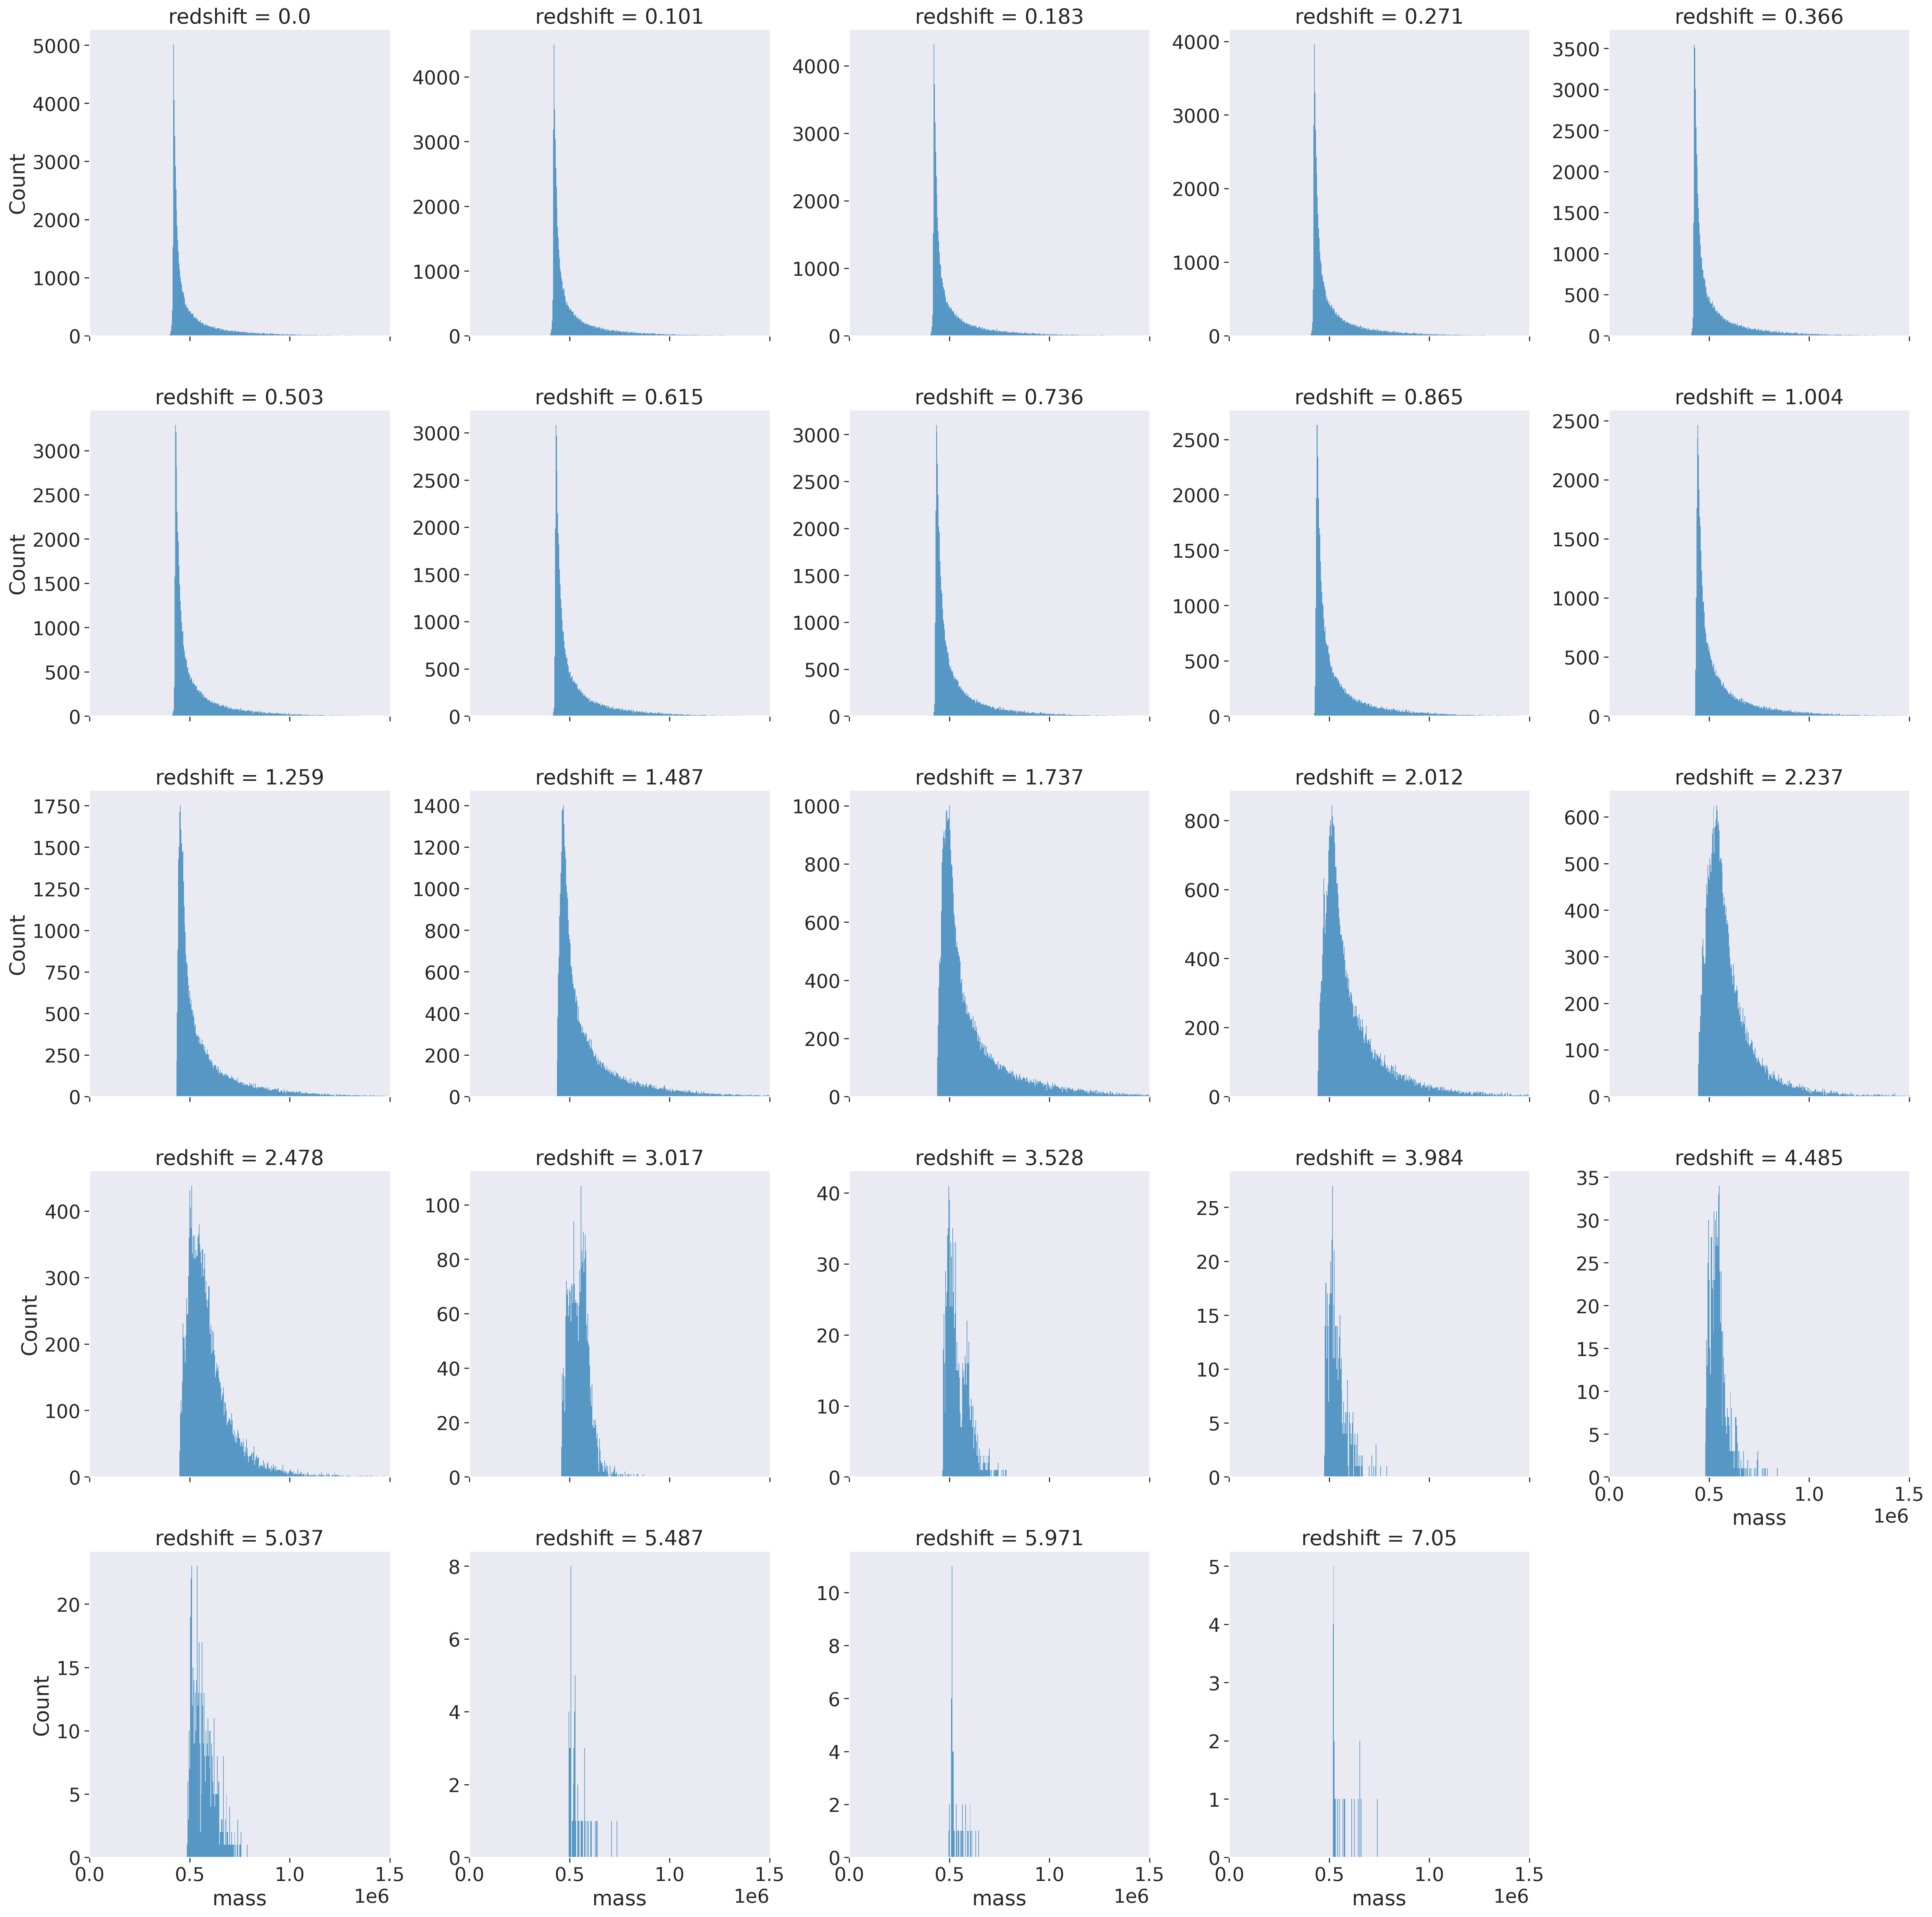
\includegraphics[width=.9\columnwidth]{../plots/mass_distribution_wrt_redshift_GM-Early.png}
			\caption{Particles mass distribution variation with redshift for GM-Early assembly mode. Note the changing y-axes scales across plots.}
	\end{figure}

	\clearpage

	\begin{figure}
			\centering 
			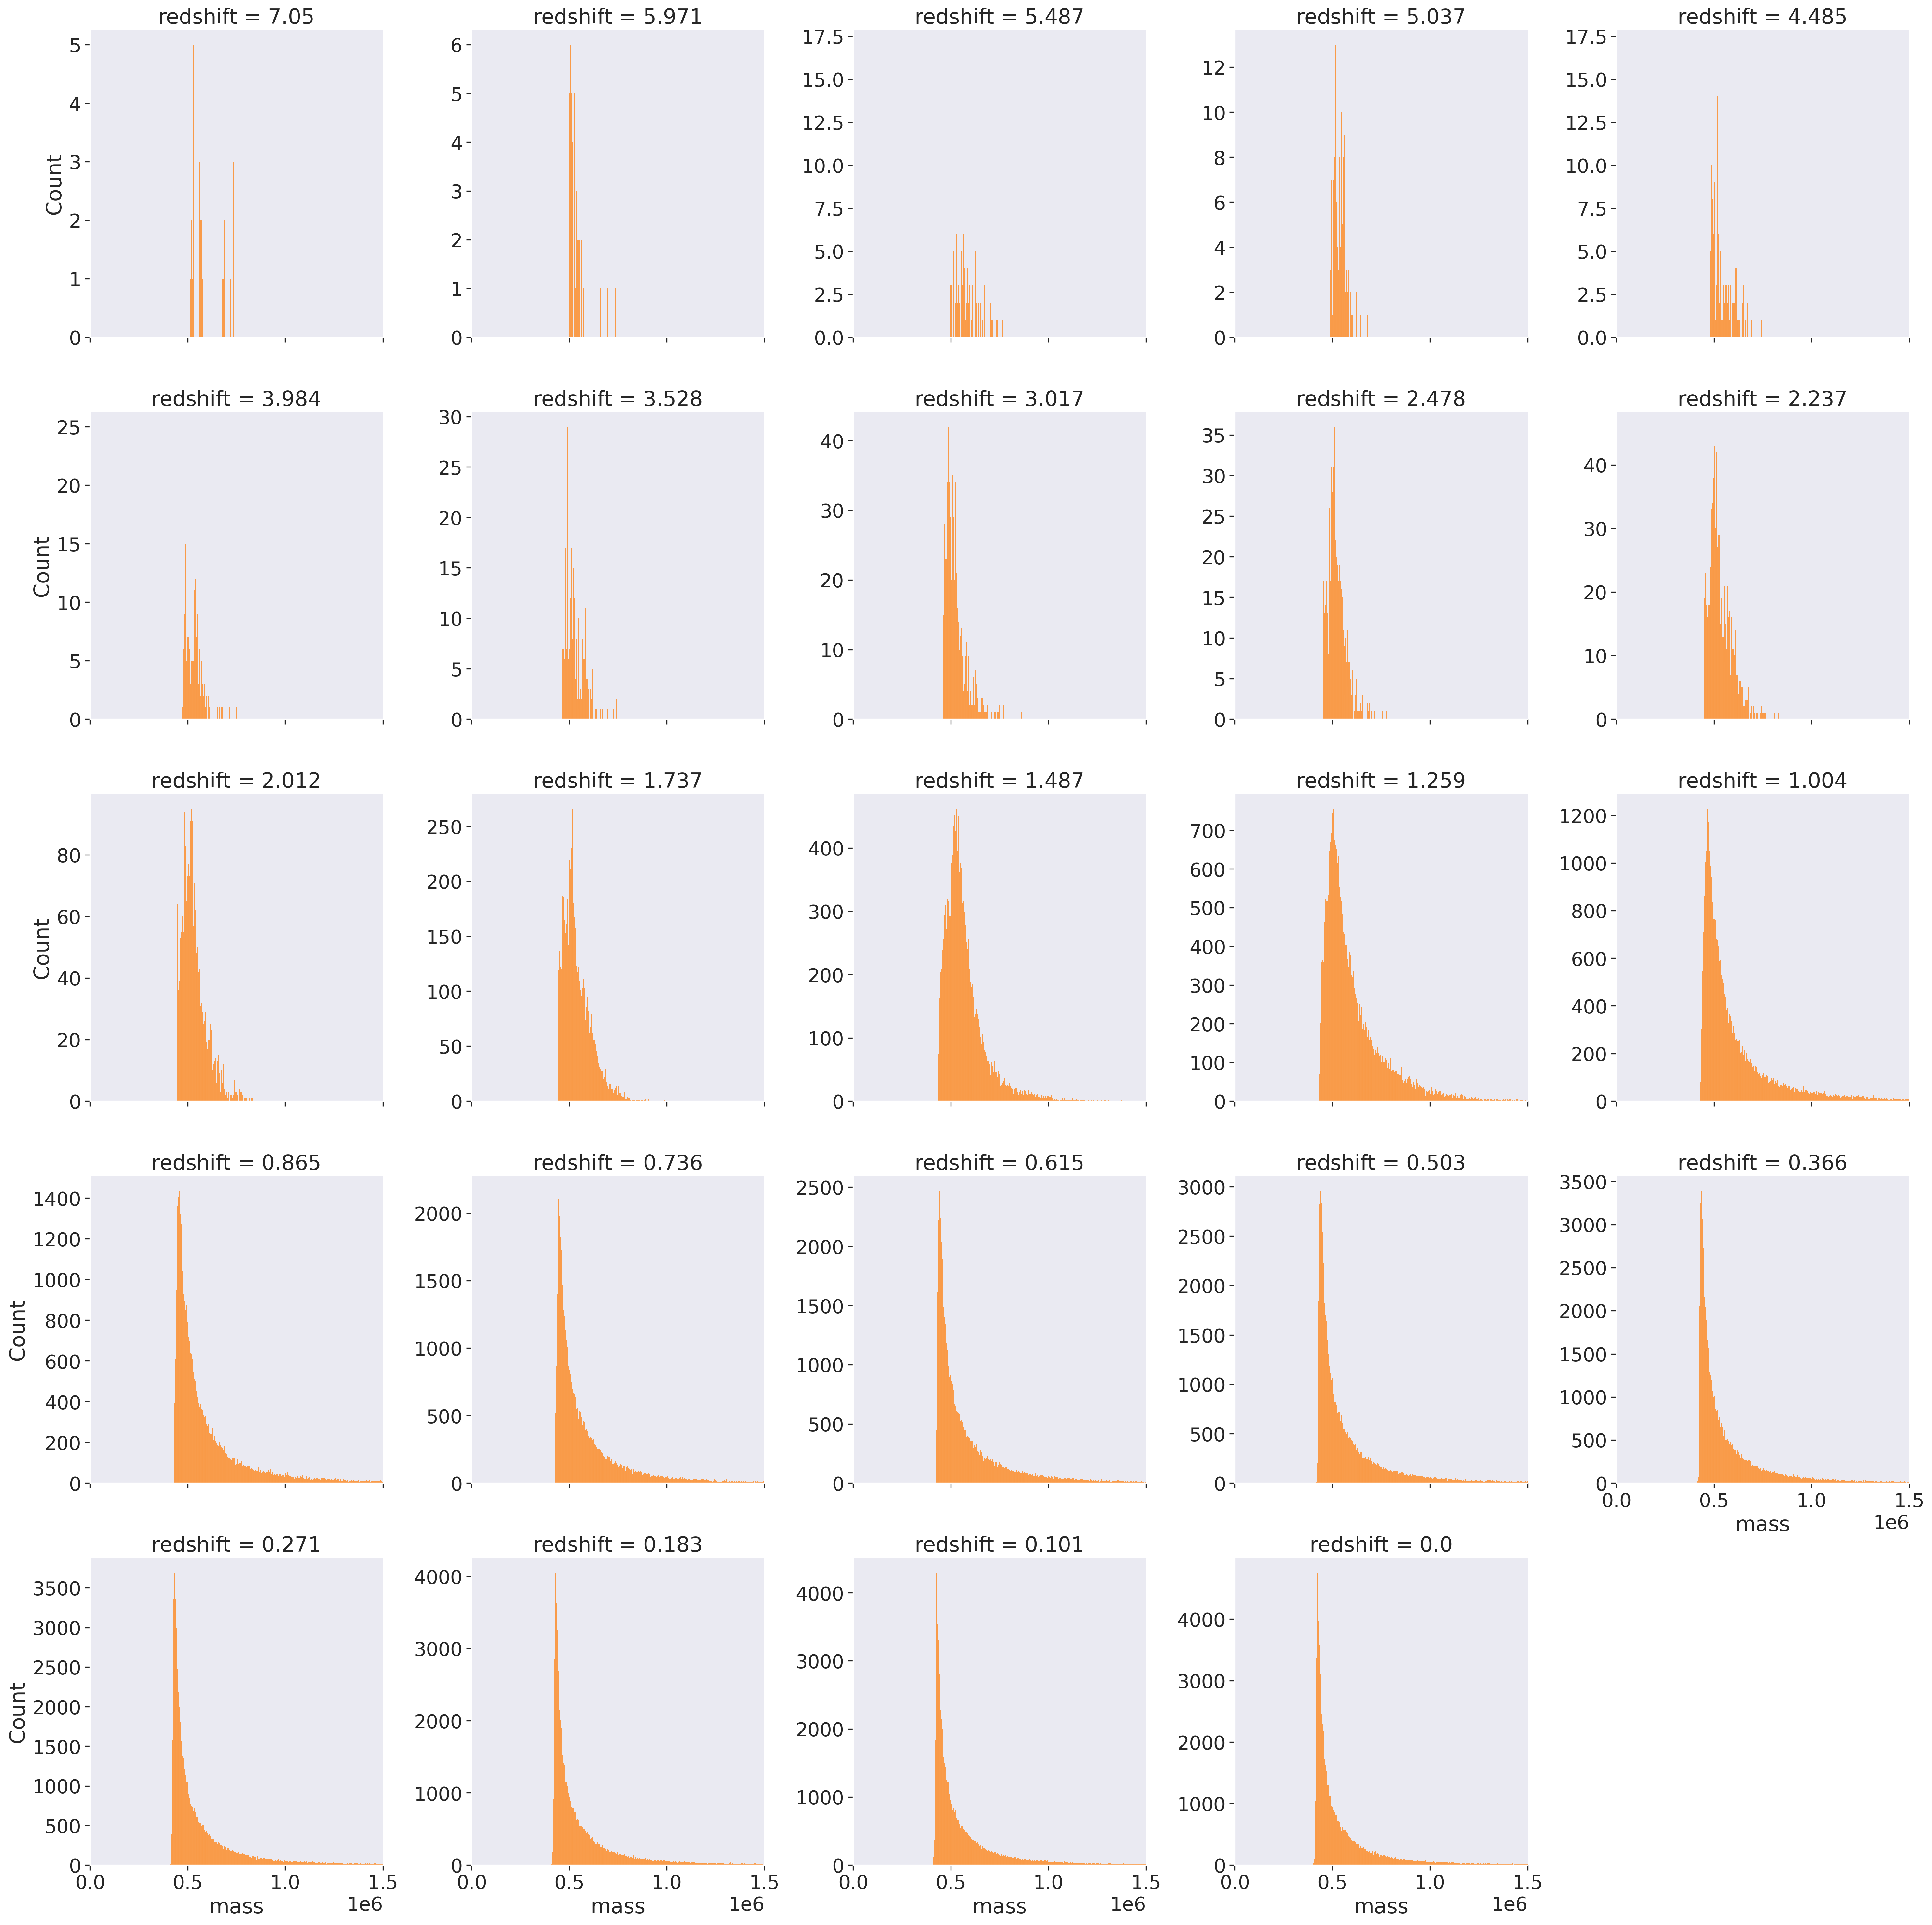
\includegraphics[width=.9\columnwidth]{../plots/mass_distribution_wrt_redshift_Organic.png}
			\caption{Particles mass distribution variation with redshift for Organic assembly mode. Note the changing y-axes scales across plots.}
	\end{figure}

	\clearpage

	\begin{figure}
			\centering 
			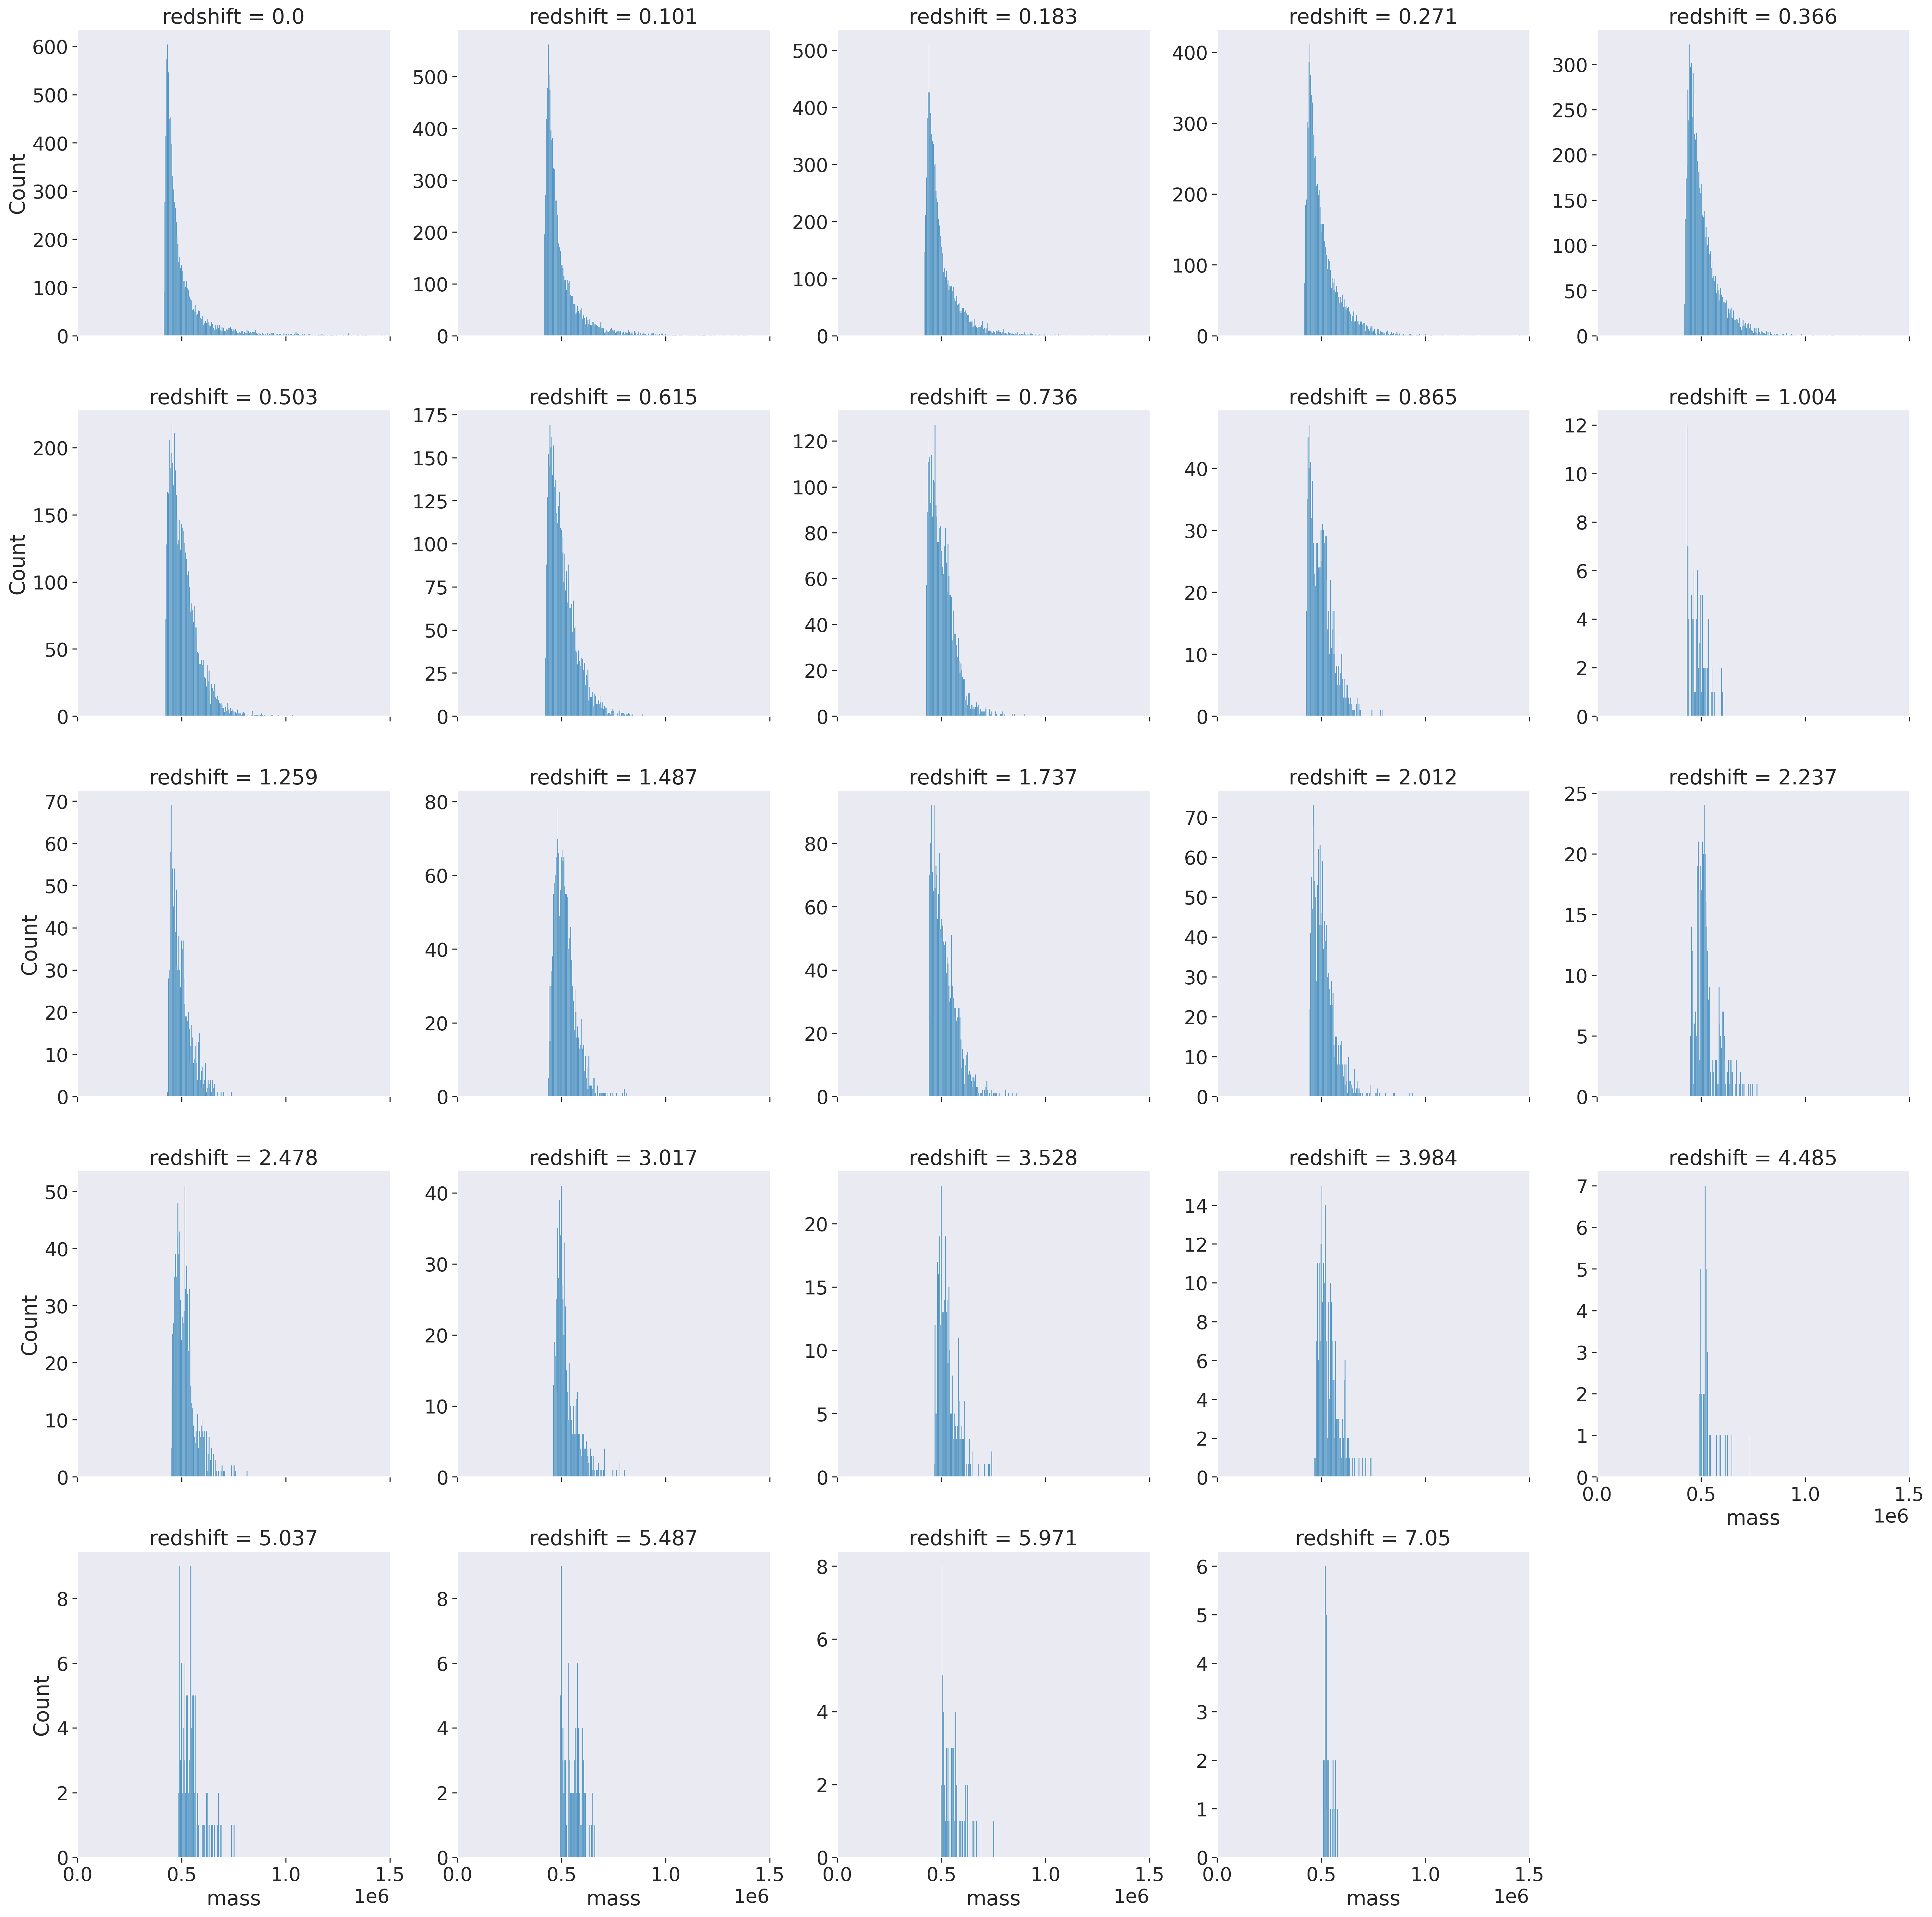
\includegraphics[width=.9\columnwidth]{../plots/mass_distribution_wrt_redshift_GM-Late.png}
			\caption{Particles mass distribution variation with redshift for GM-Late assembly mode. Note the changing y-axes scales across plots.}
	\end{figure}

\end{document}